\documentclass[10pt]{article}
\usepackage[margin=1in]{geometry}
\usepackage{booktabs}
\usepackage{graphicx}
\usepackage{amsmath,amssymb}
\usepackage[colorlinks=true,linkcolor=blue,urlcolor=blue]{hyperref}
\usepackage{xurl}

\title{Sheaf-cohomology QC for volume-EM registration:\\
pre-registered negative results and an exact view-gauge invariance}
\author{SciVizLab Vienna\thanks{Contact: [operator to fill]. v0.2, 2026-11-11; author list pending operator review.}}
\date{}

\begin{document}
\maketitle
\begin{center}\footnotesize\itshape
This work has not been peer reviewed. It is an output of an autonomous, git-frozen agent research protocol and is published as a preprint for open comment.
\end{center}

\begin{abstract}
We operationalized cohomological inconsistency (failure of adjacent-frame displacement measurements to form a $1$-coboundary on the coverage nerve) as a quality-control detector for volume-electron-microscopy registration, and evaluated it, pre-registered, on three real channels: two distant ROIs of an EMPIAR-10478 HeLa SBF-SEM block and one vendor-registered EMPIAR-10070 FIB-SEM muscle stack. Three findings survive. (1)~An \textbf{exact view-gauge invariance} (an elementary cancellation identity, stated as a remark below): whole-view displacement is an exact gauge invariance of relative-content measurement; the contribution is empirical --- a shift-channel anomaly scores AUROC exactly $0.500$ at every amplitude on real phase-correlation measurements. (2)~\textbf{Detectable bias is empirically detector-saturated within the tested closure-residual family}: an injected edge defect crosses AUROC~$0.9$ only at $\sim$4--5$\times$ the triangle-closure noise scale on raw SBF (GLR-optimal and max-abs detectors differ by $<\!0.03$; a re-implemented pairwise photometric QA baseline scores \emph{lower} than the sheaf channel at matched relative scale), while pre-registered FIB-SEM residuals sit $\sim$15$\times$ lower in absolute pixels yet still admit no $\leq\!3\times$ detection. closure-$\sigma$ scales span two orders of magnitude across techniques, a threshold sweep finds the photogrammetry prune rule budget-driven rather than rule-driven (workable $\tau$: $2.5\times$ SBF vs $3\times$ FIB-SEM at $1\%$ false flags; scoped to single-edge defects at $K{=}6$, global bundle adjustment untested), and a stitcher-free control with pixel-exact known truth reproduces the same saturation (AUROC $\leq\!0.9$ through $5\times$; view-desync exactly gauge) with detectability invariant to graph density $K\in\{5,7\}$ --- so QC thresholds must be absolute per-task tolerances, not scale-free noise multiples, and the saturation is measurement-physics, not stitching artifact. (3)~An \textbf{instrument-disclosure protocol}: a self-referential-anchor defect that flat-lined the first detector at chance was caught by an algebraic gauge proof before any gate result was seen. All results, including nulls, are frozen in git before each run; code and artifacts are public at \url{https://github.com/ScivizLabVienna/e3-sheaf-data}.
\end{abstract}

\section{Introduction}
Large volume-EM reconstructions are assembled by registering thousands of adjacent section images; registration errors propagate silently into segmentation and connectomics. Existing automated quality assessment for this step is learned and pairwise --- optical-flow SIQA metrics~\cite{emsiqa,demis}, learned features~\cite{jsee26}, vision-language judges~\cite{savior} --- and carries no structural statement about \emph{which} defects a given statistic can or cannot see.

Cellular sheaves on coverage nerves offer exactly such a statement: displacement measurements on overlaps are a $1$-cochain, a consistent registration is a coboundary, and the closure residual of every triangle is a per-edge-usable inconsistency signal with no learned parameters. Prior registration work uses the same formalism to \emph{eliminate} loop error globally (Poisson/Hodge solving)~\cite{carlino22}, never to \emph{detect} per-edge defects against a noise-calibrated threshold.

We adopted the minimal instance of this detector, pre-registered acceptance gates, and ran it on real archives. The headline outcome is negative and useful: within the tested statistics, what the detector can see is set by the channel, not by detector cleverness (we do not rule out statistics outside the closure-residual family), and the two structural claims below are exact.

\section{Formal setting}
Frames $0,\dots,N{-}1$ form a path nerve; each adjacent pair $(j,j{+}1)$ carries a measured translation $m_{jj+1}\in\mathbb{R}^2$ (phase correlation on overlapped ROIs). A \emph{closure window} of $K$ consecutive edges forms triangles whose residual is $\rho=m_{12}+m_{23}-m_{13}$ (global-reference legs measured independently at wide baseline). Two defect classes:
\textbf{M\_edge} --- a wrong offset on one edge (e.g.\ a bad correspondence patch);
\textbf{N\_shift} --- a whole-view translation desync.

\begin{quote}
\textbf{Remark (view-gauge invariance).} \emph{Adding a per-view translation $t_j$ to all measurements touching view $j$ leaves every closure residual invariant; hence no coboundary-channel statistic can discriminate an N\_shift at any amplitude.} This is an elementary cancellation identity, not a new structural result; its value here is that it predicts and explains an exactly-$0.500$ empirical null, which no learned metric can.
\end{quote}
\noindent Proof: residuals are alternating sums in which each $t_j$ appears with coefficients summing to zero. The empirical instance is exact, not approximate (\S4).

\begin{quote}
\textbf{Proposition (redundancy dilution).} \emph{In a window of $K$ edges solved by weighted least squares, one corrupted edge's offset contributes to per-row residuals at $O(1/K)$; detection difficulty grows with the very redundancy that improves fit quality.}
\end{quote}

\section{Methods (frozen before each run)}
Instrument (E6b): independent global-reference legs by wide-baseline $(+30$-frame) phase correlation plus adjacent lag-10 rows; triangle-closure residuals define $\sigma_c$ per channel, emitted \emph{before} any injection trial. Trials: $K=6$, 40 trials per class, defect levels $\{0.5,1,2,3,5\}\times\sigma_c$; detectors max-abs residual and GLR-optimal whitened $\chi^2$ energy~\cite{baarda}. Gate (identical for E6/E7/E8/E9): AUROC $\geq 0.9$ at level $\leq 3\times\sigma_c$, else detector-saturation verdict for that channel. Channels: EMPIAR-10478 SBF ROI1 (tile on disk $604{,}039{,}195$\,B, $151{\times}2000{\times}2000$), ROI2 ($740{,}048{,}035$\,B), EMPIAR-10070 FIB-SEM MITOMAP stack~\cite{mitomap} ($777{,}443{,}899$\,B, $291{\times}1595{\times}1675$, vendor TTrAC-registered). A synthetic campaign (P1--E5, oracle conditions) closed the space before real data.

\section{Results}
\begin{table}[h]\centering\small
\label{tab:mdb}
\caption{Closure $\sigma_c$ and GLR AUROC at $\{0.5,1,2,3,5\}\times\sigma_c$ (bootstrap CIs in artifacts). N\_shift: $0.500$ exactly at all levels (ROI1).}
\begin{tabular}{@{}llccccc@{}}
\toprule
Channel & $\sigma_c$ (px) & 0.5$\times$ & 1$\times$ & 2$\times$ & 3$\times$ & 5$\times$\\
\midrule
SBF ROI1 & 1.78 / 1.66 & 0.600 & 0.720 & 0.844 & 0.890 & 0.943\\
SBF ROI2 & 1.46 / 1.47 & 0.593 & 0.696 & 0.823 & 0.881 & 0.927\\
FIB-SEM  & 0.11 / 0.14 & 0.571 & 0.586 & 0.628 & 0.666 & 0.737\\
\bottomrule
\end{tabular}
\end{table}
\begin{figure}[h]\centering
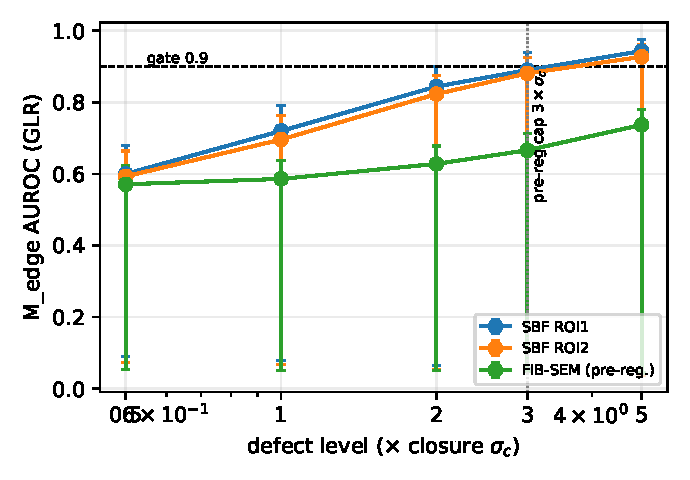
\includegraphics[width=0.72\textwidth]{fig1_mdb.pdf}
\label{fig:mdb}
\caption{MDB level curves for the injected M\_edge defect on all three channels (GLR detector; markers from the committed result artifacts, error bars are the pre-registration-frozen bootstrap CIs). The frozen gate (0.9 at $\leq 3\times$) is missed everywhere; SBF crosses between $3\times$ and $5\times$, FIB-SEM has not reached $0.9$ by $5\times$.}
\end{figure}
Table~\ref{tab:mdb} and Figure~\ref{fig:mdb} report the level curves. No channel meets the gate at $\leq 3\times$; both SBF ROIs cross $0.9$ only between $3\times$ and $5\times$ (E8 replicates E6/E7 on a distant ROI). GLR energy beats max-abs by $\leq +0.025$ AUROC everywhere; a re-implemented pairwise photometric QA baseline (EMSIQA/OFSIQA recipe~\cite{emsiqa,demis}; $360$ clean ROI1 pairs) scores \emph{worse}, AUROC $0.53$ at $3\times$. Detector design adds little \emph{within the tested family}; statistics outside it remain open. FIB-SEM inverts the mechanism --- vendor pre-registration drives $\sigma_c$ two orders of magnitude down, and redundancy dilution (Proposition) plus absolute-scale mismatch leave AUROC $<\!0.9$ even at $5\times$. \emph{Closure-$\sigma$ self-calibration does not normalize detection across channels.}

\section{Discussion}
\textbf{Operational rule.} The field practice of pruning registration residuals above $2$--$3\times$RMS~\cite{wang14} implicitly assumes noise-dominated channels. Our threshold sweep (GLR energy, hard flag at $\tau\times$null-RMS, $\tau\in\{1.5,\dots,4\}$, 86/120/226 calibration windows per channel) shows the practice is \emph{budget-driven, not rule-driven}: a $2$--$3\times$ prune catches $53$--$74\%$ of injected $\leq\!3\times$ SBF defects but only at a $0.8$--$4.7\%$ false-flag rate (SBF defect residuals sit in the far chi$^2$ tail; null RMS badly underestimates it), while the same rule flags only $19$--$30\%$ of FIB-SEM defects at a comparable budget and needs $\tau{\approx}1.5\times$ just to reach $13\%$ false flags versus $\tau{\geq}2.5\times$ on SBF: no universal $\tau$ transfers, and the operative dial is the tolerated false-flag rate, not a noise multiple. Thresholds must be absolute per-task tolerances. The same caveat applies to calibration of learned QA metrics~\cite{emsiqa,savior}.

\textbf{Disclosure protocol.} The first E6 instrument contained a self-referential-anchor defect that made the tested statistic an exact gauge by construction (AUROC flat $0.500$). It was diagnosed algebraically and disclosed \emph{before} any gate verdict; the rebuilt instrument (independent global legs) reproduced theory. We report this as a methodological contribution for agent-run science.

\textbf{Limitations.} One FIB-SEM stack (no ROI variety); no independent ground truth on EMPIAR-10070 (shifts baked by NEWSTACK; extended header byte-verified history-only), so the oracle-ceiling comparison was run only on SBF legs; serial-section TEM and array tomography untested. $\sigma_c$ on the FIB-SEM channel may partly reflect TTrAC smoothing (single stack, $n{=}1$): the stitcher-free known-truth control (E12) removes stitching as a confounder for saturation, but acquisition-side smoothing per se remains unresolved --- that channel's $\sigma_c{\approx}0.1$\,px sits below the ${\sim}0.9$\,px phase-correlation floor measured on SBF texture under known truth, which we cannot fully account for.

\section{Related work}
Hodge/Poisson elimination of loop error in global registration~\cite{carlino22}; EM stitching QA: EMSIQA~\cite{emsiqa}, OFSIQA/DEMIS~\cite{demis}, learned features~\cite{jsee26}, VLM judges~\cite{savior}; sheaf-inconsistency mathematics: consistency radius~\cite{robinson22}; streaming $H^1$~\cite{h1inc}. None evaluates coboundary residuals as calibrated per-edge QC, and none reports pre-registered negative results for volume EM.

\section{Reproducibility}
Git-campaign record (every gate dated before its run), frozen evaluators, result artifacts and bootstrap CIs: \url{https://github.com/ScivizLabVienna/e3-sheaf-data}; source data by byte-size-verified EMPIAR accessions. Rebuild: \texttt{e6b\_measure.py} $\rightarrow$ \texttt{e7\_glr.py} (numpy/scipy/tifffile).

\begin{thebibliography}{9}
\bibitem{baarda} Baarda, A. (1968). \emph{The Construction of the Adjustment of Network Models}. Delft. --- MDB and data snooping origin; photogrammetry prune practice~\cite{wang14}.
\bibitem{carlino22} Carlino, L., et al.\ (2022). Global point cloud registration by Hodge--Helmholtz. arXiv:2208.07103.
\bibitem{demis} Silling, P., et al.\ (2025). DEMIS: EM image stitching with deep features and global optimisation. SciTePress 133149; OFSIQA metric.
\bibitem{emsiqa} Shi, F., et al.\ (2024). Two-stage error detection to improve EM image mosaicking. NSF PAR 10578414.
\bibitem{jsee26} Chen, H., et al.\ (2026). Automated quality assessment of serial-section EM registration using learned features. doi:10.23919/jsee.2026.000050.
\bibitem{savior} Chen, H., et al.\ (2025). SAVIOR: volume alignment quality assessment with large vision-language models. doi:10.1016/j.neucom.2025.132038.
\bibitem{mitomap} Glancy, M., et al.\ (2015). MITOMAP FIB-SEM (EMPIAR-10070). \emph{Nature} 524:226.
\bibitem{robinson22} Robinson, M. (2022). The consistency radius for sheaves of pseudometric spaces. arXiv:2203.14057.
\bibitem{h1inc} (2026). Incremental sheaf cohomology on cellular complexes. arXiv:2606.04227.
\bibitem{wang14} Wang, Q., et al.\ (2014). Mosaicking residual pruning. ISPRS Annals II-1-C22; doi:10.5194/isprsannals-II-1-37-2014.
\end{thebibliography}

\end{document}
